\documentclass[9pt]{article}
\usepackage{fullpage}
\usepackage{amsmath}
\usepackage{amssymb}
\usepackage{graphics}
\usepackage[usenames]{color}
\usepackage{hyperref}
\usepackage{graphicx,wrapfig}
\usepackage{wallpaper}

\newcommand{\addphoto}[2]{%
  \smash{%
    \makebox[0pt][l]{%
      \raisebox{#1mm}{%
        \hspace{#2mm}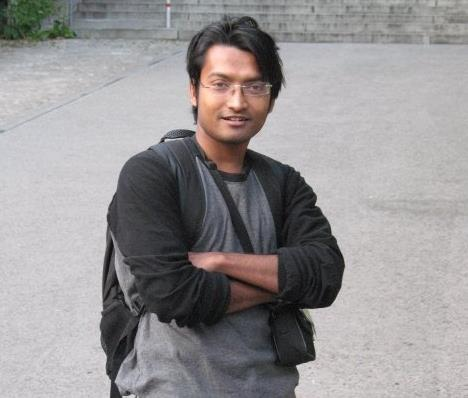
\includegraphics[scale=1]{mypic_1}%
      }%
     }%
  }%
}
\hypersetup{
    colorlinks=true,
    citecolor=blue,%
    filecolor=blue,%
    linkcolor=blue,%
    urlcolor=blue
}


\leftmargin=0.25in
\oddsidemargin=0.25in
\textwidth=6.0in
\topmargin=-0.25in
\textheight=9.25in
\newcommand{\p}{p{8cm}}

\raggedright

\pagenumbering{arabic}

\def\bull{\vrule height 0.8ex width .7ex depth -.1ex }
% DEFINITIONS FOR RESUME

\newenvironment{changemargin}[2]{%
  \begin{list}{}{%
    \setlength{\topsep}{0pt}%
    \setlength{\leftmargin}{#1}%
    \setlength{\rightmargin}{#2}%
    \setlength{\listparindent}{\parindent}%
    \setlength{\itemindent}{\parindent}%
    \setlength{\parsep}{\parskip}%
  }%
  \item[]}{\end{list}
}

\newcommand{\lineover}{
	\begin{changemargin}{-0.05in}{-0.05in}
		\vspace*{-8pt}
		\hrulefill \\
		\vspace*{-2pt}
	\end{changemargin}
}

\newcommand{\header}[1]{
	\begin{changemargin}{-0.5in}{-0.5in}
		\scshape{#1}\\
  	\lineover
	\end{changemargin}
}

\newcommand{\cmnt}[1]{}

\newcommand{\contact}[4]{
	\begin{changemargin}{-0.5in}{-0.5in}
		\begin{center}
			{\Large \scshape {#1}}\\ \smallskip
			{#2}\\ \smallskip 
			{#3}\\ \smallskip
			{#4}\smallskip
		\end{center}
	\end{changemargin}
}

\newenvironment{body} {
	\vspace*{-16pt}
	\begin{changemargin}{-0.25in}{-0.5in}
  }	
	{\end{changemargin}
}	

\newcommand{\school}[4]{
	\textbf{#1} \hfill \emph{#2\\}
	#3\\ 
	#4\\
}

% END RESUME DEFINITIONS

\begin{document}

%%%%%%%%%%%%%%%%%%%%%%%%%%%%%%%%%%%%%%%%%%%%%%%%%%%%%%%%%%%%%%%%%%%%%%%%%%%%%%%%
% Name
	\begin{changemargin}{-0.5in}{-0.5in}
\begin{tabular}{lr}
\begin{tabular}{c}
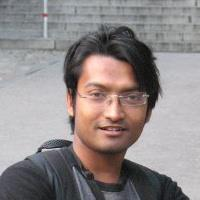
\includegraphics[height=35mm,width=35mm]{mypic3.png}
\end{tabular} & 
\begin{tabular}{c}
\\ \\  
\qquad\qquad\qquad\qquad\qquad\qquad\quad {\Large Sandeep Dasgupta} \\ 
\begin{tabular}{l}
\qquad\qquad\qquad\qquad\qquad\qquad\qquad {{\texttt{email}: sdasgup3 [at] cs [dot] illinois [dot] edu}} \\
\qquad\qquad\qquad\qquad\qquad\qquad\qquad {{\texttt{url}: \url{http://web.engr.illinois.edu/~sdasgup3}}} \\
\qquad\qquad\qquad\qquad\qquad\qquad\qquad {{\texttt{phone}: (+1) 2174172344}} \\
\end{tabular}  
\end{tabular} \\
&\\
\end{tabular} 

	\end{changemargin}


%%%%%%%%%%%%%%%%%%%%%%%%%%%%%%%%%%%%%%%%%%%%%%%%%%%%%%%%%%%%%%%%%%%%%%%%%%%%%%%%
% Objective
\header{Research Interest}

\begin{body}
	\vspace{14pt}
		Compiler Optimizations \\
		Static Program Analysis \& Verification \\
                Symbolic Execution \\                
		Parallel \& Power Aware Computation \\
%		Parallel Computing \\
%		Programming Language Design \& Implementation \\
% 		Automated software verification \& quality assurance.
\end{body}

\smallskip


%%%%%%%%%%%%%%%%%%%%%%%%%%%%%%%%%%%%%%%%%%%%%%%%%%%%%%%%%%%%%%%%%%%%%%%%%%%%%%%%
% Education
\header{Academics}

\begin{body}
	\vspace{14pt}
	\textbf{PhD Computer Science }{} \hfill \emph{August 2013 - untill now}{} \\
	\emph{\href{http://cs.illinois.edu/}{CS @ University of Illinois Urbana Champaign}}{} \\
	\begin{itemize} \itemsep -0pt
		\item Currently working with \href{http://llvm.org/}{ LLVM Group} led by Prof. \href{http://web.engr.illinois.edu/~vadve/Home.html}{Vikram S. Adve}
	\end{itemize}
 \medskip
	\textbf{M.Tech Computer Science \& Engineering -- CPI 9.00/10.00}{} \hfill \emph{August 2009 - June 2011}{} \\
	\emph{\href{http://www.iitk.ac.in/}{Indian Institute Of Technology Kanpur}, Kanpur, India.}{} \\
	\begin{itemize} \itemsep -0pt
		\item Secured \textbf{rank $1$} in M. Tech 2009 Batch, IIT Kanpur.
	\end{itemize}
  \medskip
	\textbf{B.E. Computer Science \& Engineering -- \emph{First Class with Honours}, 85.625/100.00} \hfill \emph{August 2002 - June 2006} \\
	\emph{\href{http://www.becs.ac.in/}{Bengal Engineering \& Science University, Shibpur}}, West Bengal, India.\\
	\begin{itemize} \itemsep -0pt
		\item Awarded \textbf{University Gold Medal} for securing 1st Rank in BE, Computer Science \& Engineering, 2002 batch.
		\item Awarded \textbf{Best Student Award}, sponsored by \href{http://www.tcs.com}{Tata Consultancy Services}, for outstanding performance in BE, Computer Science \& Engineering, 2002 batch.
	\end{itemize}
\end{body}

\smallskip

%%%%%%%%%%%%%%%%%%%%%%%%%%%%%%%%%%%%%%%%%%%%%%%%%%%%%%%%%%%%%%%%%%%%%%%%%%%%%%%%
% Courses and Projects
\header{Graduate Courses \& Projects}

\begin{body}
	\vspace{14pt}
	\textbf{Graduate Courses }{} \hfill \\
	\begin{itemize} \itemsep -0pt
          \item \href{https://cs.illinois.edu/courses/profile/CS526}{CS526: }Advanced Compiler Construction
          \item \href{https://courses.engr.illinois.edu/cs533/}{CS533: }Parallel Computer Architectures
          \item \href{https://wiki.cites.illinois.edu/wiki/display/cs598lvk/Home}{CS598lvk: }Parallel Programming with Migratable Objects
          \item  \href{https://cs.illinois.edu/courses/profile/CS420}{CS420/CSE402/ECE492: }
                                            Introduction to Parallel Programming for Scientists and Engineers
	\end{itemize}
 \medskip
	\textbf{Projects}{} \hfill  \\
	\begin{itemize} \itemsep -0pt
           \item \textbf{Partial Redundancy Elimination(PRE)} \href{https://github.com/sdasgup3/PartialRedundancyElimination}{[Github]} \\
                                  \texttt{Abstract: }PRE is a compiler optimization that
                                  eliminates expressions that are redundant on
                                  some but not necessarily all paths through a
                                  program. In this project, we implemented a PRE
                                  optimization pass in LLVM and measured results
                                  on a variety of applications. It's a powerful
                                  technique that subsumes Common Subexpression
                                  Elimination (CSE) and Loop Invariant Code
                                  Motion (LICM), and hence has a potential to
                                  greatly improve performance.  

            \item \textbf{Implementing Data flow Analyzer} \\
                                \texttt{Abstract: }To Extend the Generic Data Flow Analyzer
                                GDFA (of gcc) to the data flow frameworks where
                                data flow information can be represented using
                                bit vectors but the frameworks are not bit
                                vector frameworks because they are
                                non-separable e.g., faint variable analysis,
                                possible undefined variable analysis, strongly
                                live variable analysis.	
          \item \textbf{Mitigating Impact of Heterogeneity Across Power-constrained Nodes on Parallel Applications through Load Balancing}     
                                \href{https://github.com/sdasgup3/HeterogeneityAwareLoadBalancing}{[Github]} \\
                                  \texttt{Abstract: }Different processors across the nodes
                                  have different execution times for the same
                                  work-loads. This performance imbalance is seen
                                  only when the CPU power is capped to low
                                  values. This performance imbalance causes
                                  increased execution times of the parallel
                                  applications. We did a detailed study and
                                  proposed a power aware load balancer (using
                                      Charm++ ) which minimized the performance
                                  imbalance at the lower power caps by tackling
                                  this heterogeneity.  
           \item \textbf{Designing superscalar processor} \href{https://github.com/sdasgup3/Parallel-Processor-Design}{[Github]} \\
                                \texttt{Abstract: }To design a customized processor (using
                                    parallel processing concepts) for the
                                application of document retrieval system. We
                                developed a superscalar processor (with  an
                                    issue rate of 2) using verilog hdl, and an
                                assembler for that processor using flex and
                                bison.  

           \item \textbf{Graph Coloring Using State Space Search} \href{https://github.com/sdasgup3/ParallelSudoku}{[Github]} \\          
                                  \texttt{Abstract: }We plan to leverage the state space
                                  search model for implementing graph coloring
                                  in parallel in Charm++. Some of the
                                  challenges for efficient exploration of space
                                  by chares include intelligent pruning of the
                                  state space, load balancing, grain-size
                                  control and low-overhead communication
                                  between chares. We evaluated multiple options
                                  for each of these, and come up with design
                                  decisions which would work for a large
                                  category of real-life graph applications.
	\end{itemize}
\end{body}

\smallskip

%%%%%%%%%%%%%%%%%%%%%%%%%%%%%%%%%%%%%%%%%%%%%%%%%%%%%%%%%%%%%%%%%%%%%%%%%%%%%%%%
% MTech Thesis
\header{M.Tech Thesis \hfill Joint supervision of \href{http://www.cse.iitk.ac.in/users/karkare/}{Dr. Amey karkare} \& \href{http://www.cse.iitk.ac.in/users/ska/}{Dr.  Sanjeev K Aggarwal} }

\begin{body}
	\vspace{14pt}
	\textbf Precise Shape Analysis Using Field Sensitivity {\href{http://www.cse.iitk.ac.in/users/karkare/MTP/2010-11/sandeep2010precise.pdf}{[Report]}} \\
		\begin{itemize} \itemsep -0pt  
		\item[] To disambiguate heap allocated data-structures by estimating the shape (Tree, Dag or Cyclic Graph ) of the data structure 
			accessible from each heap directed pointer. This will help in automatic parallelization of sequential code having heap 
			intensive data structures. The work mainly focuses on devising a novel shape analysis technique. 
		\end{itemize}
\end{body}

\smallskip

% Publications
\header{Publications}
\begin{body}
\vspace{14pt}
\textbf{Papers in Conferences}\\
	\vspace*{-4pt}
	\begin{itemize} \itemsep -0pt
		\item Sandeep Dasgupta \& Amey Karkare.``\textbf{Precise shape analysis using field sensitivity}'', in \emph{Proceedings of the 27th Annual ACM Symposium on Applied Computing}, SAC 2012, pages 1300-1307, New York, USA. ACM. \href{http://dx.doi.org/10.1145/2245276.2231982}{doi: 10.1145/2231936.2231982}, isbn: 978-1-4503-0857-1. \href{https://dl.dropbox.com/u/86719354/sac\_2012.pdf}{[pdf]}\\

		\item Barnali Basak, Sandeep Dasgupta \& Amey Karkare.``\textbf{Heap Dependence Analysis for Sequential Programs}'', \emph{International Conference on Parallel Computing} (ParCo 2011), Ghent, Belgium, August 30 - September 2, 2011. \href{https://dl.dropbox.com/u/86719354/parco\_2011.pdf}{[pdf]} \\
		\begin{itemize} \itemsep -0pt
			\item Published in: Applications, Tools and Techniques on the Road to Exascale Computing, 22 volume of Advances in 
				Parallel Computing, chapter: Heap Dependence Analysis for Sequential Programs, pages 99--106. IOS Press, May 2012. 
				doi: \href{http://dx.doi.org/10.3233/978-1-61499-041-3-99}{10.3233/978-1-61499-041-3-99}, isbn: 978-1-61499-040-6.
		\end{itemize}
	\end{itemize}

\textbf{Posters}\\
	\vspace*{-4pt}
	\begin{itemize} \itemsep -0pt
		\item Poster ``\textbf{Dependence Analysis for Parallelization 
		of Sequential Programs}'' got accepted at APLAS`10 (the 8th ASIAN Symposium on Programming Languages \& Systems). \href{https://dl.dropbox.com/u/86719354/poster_APLAS2010.pdf}{[pdf]}
	\end{itemize}

\textbf{Journals}\\
	\vspace{-4pt}
	\begin{itemize} \itemsep -0pt
		\item  Sandeep Dasgupta, Amey Karkare \& P.\ Vinay K.\ Reddy. ``\textbf{Precise shape analysis using field sensitivity}.'', in \emph{Innovations in Systems and Software Engineering (ISSE)}, a NASA journal.
                 doi: \href{http://www.springerlink.com/openurl.asp?genre=article&id=doi:10.1007/s11334-013-0198-7}{10.1007/s11334-013-0198-7}. \href{https://dl.dropbox.com/u/86719354/publication_isse.pdf}{[pdf]}
	\end{itemize}
\end{body}

%%%%%%%%%%%%%%%%%%%%%%%%%%%%%%%%%%%%%%%%%%%%%%%%%%%%%%%%%%%%%%%%%%%%%%%%%%%%%%%%
%Professional Experience
\header{Professional Experience}

\begin{body}
	\vspace{14pt}
	\href{http://www.intel.in/content/www/in/en/homepage.html}{\textbf{Intel Technology India Pvt. Ltd.}}, \emph{Component Design Engineer} \hfill \emph{August 2011 - June 2013}\\
	\vspace*{-4pt}
	\begin{itemize} \itemsep -0pt  % reduce space between items
                \item Worked as Design Automation Engineer for Formal Equivalence Verification of hardware designs.
                \item Contributed to and supported Broadwell (BDX) and Skylake (SKL) FEV requirements. Played key role in FEV audit checks for BDX. 
                \item Owner of tools and infrastructures for driving
                FEV central runs for  BDX. Worked closely with teams of various
                design styles in understanding the requirements for
                customization and also provided the much needed support for
                successfully deploying those tools.
                \item Build flows and methodologies to provide solutions on how
                to formally verify leading next generation CPU designs.
                Interacted closely with global FEV teams to understand the
                requirements and contributed to the success of various
                sprints with timely and quality delivery on assignments.
                \end{itemize}

	\href{http://www.interrasystems.com/}{\textbf {Interra Systems India Pvt. Ltd.}}, \emph{Senior Member Of Technical Staff} \hfill \emph{August 2006 - July 2009}\\
	\vspace*{-4pt}
	\begin{itemize} \itemsep -0pt
		\item Developer of Interra's premiere front-end analyzer products - Cheetah (SystemVerilog) and MVV(Mixed Verilog Vhdl) and 
		provided support for several new constructs of System Verilog IEEE-1800-2005, fixed tool bugs, created applications and contributed in performance Improvement. 		
		\item Involved in a critical service project for \href{http://www.atrenta.com/}{Atrenta (I) Pvt. Ltd.} for the development of System Verilog features in Spyglass DFT.
	\end{itemize}
\end{body}

\smallskip

%%%%%%%%%%%%%%%%%%%%%%%%%%%%%%%%%%%%%%%%%%%%%%%%%%%%%%%%%%%%%%%%%%%%%%%%%%%%%%%%
%Teaching Experience
\header{Teaching Experience}

\begin{body}
	\vspace{14pt}
	\textbf{University Of Illinois Urbana Champaign},  \hfill \emph{August 2013 - December 2013}\\
	\vspace*{-4pt}
	\begin{itemize} \itemsep -0pt  % reduce space between items
		\item \textbf{Teaching Assistant} for \href{http://cs.illinois.edu/courses/profile/CS427-120138}{CS 427: Software Engineering I}: A Graduate level course.
			\begin{itemize}
				\item Designing the questions for homework and term examinations and grading those.
				\item Conducting discussion sessions with the students to answer questions related to lectures/homework.   
			\end{itemize}
	\end{itemize}

	\textbf{Indian Institute of Technology, Kanpur},  \hfill \emph{August 2009 - 2011}\\
	\vspace*{-4pt}
	\begin{itemize} \itemsep -0pt  % reduce space between items
		\item \textbf{Tutor} for \href{http://www.cse.iitk.ac.in/teaching/courses/ESc101.html}{ESc 101: Fundamentals of Computing}: An undergraduate course.
			\begin{itemize}
				\item Responsible for weekly lecture class on C - programming language, supervision of programming laboratory and grading assignments and term examinations.
			\end{itemize}
		\item \textbf{Teaching Assistant} for \href{http://www.cse.iitk.ac.in/teaching/courses/CS335.html}{CS 335: Principles of Compiler Design}: An undergraduate course.
			\begin{itemize}
				\item Responsible for mentoring a student group on a course project of developing a simple compiler (using a subset of C-language constructs) demonstrating most of the phases of compiler design starting from Lexical \& Syntax analysis upto Intermediate code generation.
				\item Grading assignments and term examinations.
			\end{itemize}
		\item \textbf{Teaching Assistant} for \href{http://www.cse.iitk.ac.in/teaching/courses/CS355.html}{CS355: Programming Tools and Techniques}: An undergraduate course.
			\begin{itemize}
				\item Grading assignments related to Software management tools such as make; Programming tools such as Python, Perl; Document preparation systems such as tex; Tools for building programs like Lex and Yacc.
			\end{itemize}
	\end{itemize}
\end{body}

\smallskip
%%%%%%%%%%%%%%%%%%%%%%%%%%%%%%%%%%%%%%%%%%%%%%%%%%%%%%%%%%%%%%%%%%%%%%%%%%%%%%%%

% Awards and Honors
\header{Achievements/Distinctions}

\begin{body}
	\vspace{14pt}
	\begin{itemize} \itemsep -0pt  % reduce space between items
		\item Awarded \textbf{University Gold Medal} for securing 1st Rank in BE, Computer Science \& Engineering, 2002 batch.\\
		\item Awarded \textbf{Best Student Award}, sponsored by \href{http://www.tcs.com}{Tata Consultancy Services}, for outstanding performance in BE, Computer Science \& Engineering, 2002 batch. \\
		\item \textbf{Secured Rank $1$}, in M. Tech 2009 Batch, IIT Kanpur.
		\item \textbf{Secured All India Rank $145$} (99.64 percentile) in GATE 2009, an exam for admission in Graduate Study.
		\item \textbf{Ranked $356^{th}$} (among $\frac{1}{10}$ of Million+ students) in WB-JEE, 2002, an exam for admission in undergraduate study.
		\item Awarded \textbf{Interra Humming Bird Award} in recognition of \& appreciation for providing excellent support to \href{}{Atrenta (I) Pvt. Ltd.} in the project ``IEEE compliance for Spyglass'', awarded by \href{http://www.interrasystems.com/}{Interra Systems India Pvt. Ltd.} 
	\end{itemize} 
\end{body}

\smallskip



\end{document}


\cmnt{
%%%%%%%%%%%%%%%%%%%%%%%%%%%%%%%%%%%%%%%%%%%%%%%%%%%%%%%%%%%%%%%%%%%%%%%%%%%%%%%%
% MTech Course Projects
\header{M.Tech Course Projects}

\begin{body}
	\vspace{14pt}
	\textbf{\href{http://www.cse.iitk.ac.in/teaching/courses/CS738.html}{Advanced Compiler Optimizations}} \\
		\begin{itemize} \itemsep -0pt 
			\item[] To Extend the Generic Data Flow Analyzer GDFA (of gcc) to the data flow frameworks where data flow information can
				be represented using bit vectors but the frameworks are not bit vector frameworks because they are non-separable e.g.,
				faint variable analysis, possible undefined variable analysis, strongly live variable analysis.
		\end{itemize}

  		\medskip

	\textbf{\href{http://www.cse.iitk.ac.in/teaching/courses/CS633.html}{Parallel Computing}} \\
		\begin{itemize} \itemsep -0pt 
			\item[] To design a customized processor (using parallel processing concepts) for the application of document retrieval
				system. We developed a \href{https://github.com/sdasgup3/Parallel-Processor-Design}{superscalar processor (with  an issue rate of 2)} using verilog hdl, and an assembler for that processor using flex and bison.
		\end{itemize}
\end{body}

\smallskip
\newpage

%%%%%%%%%%%%%%%%%%%%%%%%%%%%%%%%%%%%%%%%%%%%%%%%%%%%%%%%%%%%%%%%%%%%%%%%%%%%%%%%
% BTech Course Projects
\header{B.Tech Project \hfill under supervision of \href{http://cse.iitkgp.ac.in/~pb}{Dr. Partha Bhowmick}}

\begin{body}
	\vspace{14pt}
	\textbf{\href{http://dl.dropbox.com/u/86719354/BE_project.pdf}{Affine Transformation of Digital Curves Using Chain Codes.}}  \\
		\begin{itemize} \itemsep -0pt  
		\item[]  Affine Transformation of Digital Curves Using Chain Codes. The problem statement is to rotate a digital image by a given angle.
		\end{itemize}
\end{body}

\smallskip
\smallskip

%%%%%%%%%%%%%%%%%%%%%%%%%%%%%%%%%%%%%%%%%%%%%%%%%%%%%%%%%%%%%%%%%%%%%%%%%%%%%%%%
% References
\header{References}
	\vspace{14pt}

\begin{body}
%\begin{table}[position specifier]
%\centering
\begin{tabular}{l|l}

& \\
	\begin{tabular}{\p}
		\href{http://www.cse.iitk.ac.in/users/karkare/}{Dr. Amey Karkare}, \\
		Assistant Professor, \\
		Department Of Computer Science \& Engineering, \\
		Indian Institute Of Technology Kanpur, India. \\
		Phone:	+91 512 259 7520 (Office) \\
		Email: karkare@gmail.com, karkare@cse.iitk.ac.in	
                Mobile: 919532689131
	\end{tabular} &
	\begin{tabular}{\p}
		\href{http://cse.iitkgp.ac.in/~pb/}{Dr. Partha Bhowmick}, \\
		Professor, \\
		Department Of Computer Science \& Engineering, \\
		Indian Institute Of Technology Kharagpur, India. \\
		Phone:	+91-3222-283468 \\
		FAX:	+91-3222-278985 \\
		Email:	pb@cse.iitkgp.ernet.in \\
		gmail:	 bhowmick@gmail.com \\
	\end{tabular} \\
& \\ \hline
& \\
	\begin{tabular}{\p}
		\href{http://www.becs.ac.in/aboutjaya-sil-cstmenuitem}{Dr. Jaya Sil}, \\
		Professor, \\
		Department of Computer Science and Technology, \\
		Bengal Engineering \& Science University, Shibpure, West Bengal, India. \\
		Phone: +91 - 33 - 26684561/62/63 Ext. \\
		Email:	js@cs.becs.ac.in \\
		%Mobile: 09433283641 
	\end{tabular} &
	\begin{tabular}{\p}
	\href{http://www.linkedin.com/pub/neelu-bajaj/8/491/7a7}{Neelu Bajaj}, \\
	Director Engg. at Atrenta India Pvt. Ltd. \\
	Email: neelu@noida.atrenta.com \\
%	Mobile: (91) 9810803073.
	\end{tabular} \\ 
& \\ \hline
& \\
	\begin{tabular}{\p}
		\href{http://www.linkedin.com/pub/kausik-datta/1/9a8/964}{Kausik Datta}, \\
		Senior Manager at Mentor Graphics, \\
		Kolkata Area, India \\
		%Phone: +91 - 9830252538 \\
		Email:	datta.kausik@gmail.com \\
		%Mobile: 09433283641 
	\end{tabular} &
	\begin{tabular}{\p}
		\href{http://www.jaduniv.edu.in/profile.php?uid=615}{Dr. Samiran Chattopadhyay}, \\
		Head Of The Department, \\ 
		\href{http://www.jaduniv.edu.in/view\_department.php?deptid=90}{Department of Information Technology}, \href{http://www.jaduniv.edu.in/}{Jadavpur University}, \\
		West Bengal, India. \\
		PH: 2335-8321 (O), 2414-6666 \\
		Email:	samirancju@gmail.com \\
		Mobile: 91 9830613450
	\end{tabular} \\
& \\ \hline

\end{tabular}
	
\end{body}
}
